
\section{Auswertung}
Zunächst werden die gemessenen Werte in einer Tabelle dargestellt.
Diese ist in Tabelle (\ref{tab:1}) zu sehen.

\begin{table}
  \centering
  \caption{gemessene Werte}
  \label{tab:1}
  \begin{tabular}{c c c c c c c c}
    \toprule $Zeit[s]$ & $T_1[°C]$ & $T_1[K]$ &  $p_a[bar]$ & $T_2[°C]$ & $T_2[K]$ &
    $p_b[bar]$ & $N[W]$\\
    \midrule
    0   & 20,2 & 293,35 & 5,1 & 20,2 & 293,35 & 5,5  & 170 \\
    60  & 22,3 & 295,45 & 2,8 & 20,2 & 293,35 & 7,5  & 173 \\
    120 & 23,8 & 296,95 & 3,0 & 19,4 & 292,55 & 8,0  & 185 \\
    180 & 26,2 & 299,35 & 3,1 & 18,0 & 291,15 & 8,5  & 195 \\
    240 & 28,7 & 301,85 & 3,1 & 16,2 & 289,25 & 9,0  & 200 \\
    300 & 31,4 & 304,55 & 3,1 & 14,4 & 287,55 & 9,5  & 204 \\
    360 & 33,7 & 306,85 & 3,1 & 12,7 & 285,85 & 10,0  & 206 \\
    420 & 31,5 & 304,65 & 3,1 & 11,0 & 284,15 & 9,25 & 206 \\
    480 & 33,4 & 306,55 & 3,1 &  9,5 & 282,65 & 9,5  & 203 \\
    540 & 35,4 & 308,55 & 3,1 &  7,6 & 280,75 & 10,0  & 207 \\
    600 & 37,2 & 310,35 & 3,1 &  6,0 & 279,15 & 10,25 & 210 \\
    660 & 38,9 & 312,05 & 3,1 &  4,5 & 277,65 & 10,75 & 210 \\
    720 & 40,7 & 313,85 & 3,1 &  2,7 & 275,85 & 11,0 & 210 \\
    780 & 42,2 & 315,35 & 3,1 &  1,5 & 274,65 & 11,5 & 212 \\
    840 & 43,9 & 317,05 & 3,1 &  0,6 & 273,75 & 12,0 & 212 \\
    900 & 45,4 & 318,55 & 3,1 & -0,2 & 272,95 & 12,5 & 210 \\
    960 & 46,8 & 319,95 & 3,1 & -0,7 & 272,45 & 12,5 & 210 \\
    1020& 48,2 & 321,35 & 3,1 & -1,0 & 272,15 & 13,0 & 208 \\
    1080& 49,4 & 322,55 & 3,1 & -1,4 & 271,75 & 13,5 & 204 \\
    1140& 50,5 & 323,65 & 3,1 & -1,8 & 271,35 & 14,0 & 204 \\
    \bottomrule
  \end{tabular}
\end{table}
\subsection{Temperaturverlauf}
Um den Temperaturverlauf darzustellen,
werden die gemessenen Werte für die Temperatur gegen die Zeit augetragen.
Dies ist in Abbildung (\ref{fig:temp})
Mit der Funktion:
\begin{equation*}
  T(t) = At^2 + Bt +C
\end{equation*}
 wird eine Ausgleichsrechnung durchgeführt.
 Die Parameter $A$, $B$ und $C$ werden mittels python bestimmt und lauten:\\
 \emph{Für $T_1$}:
 \begin{align*}
   A &= (-3,8 \pm 2,0)\cdot 10^{-6} \, \mathrm{\frac{K}{s^2}} \\
   B &= (0,0306 \pm 0,0023) \, \mathrm{\frac{K}{s}} \\
   C &= (293,9 \pm 0,6 )\, \mathrm{K}
 \end{align*}
 \emph{für $T_2$}:
 \begin{align*}
   A &= (9,0 \pm 2,0)\cdot 10^{-6}\, \mathrm{\frac{K}{s^2}} \\
   B &= (-0,0325 \pm 0,0024)\, \mathrm{\frac{K}{s}} \\
   C &= (295,6 \pm 0,6)\, \mathrm{K}
 \end{align*}

 \begin{figure}
   \centering
   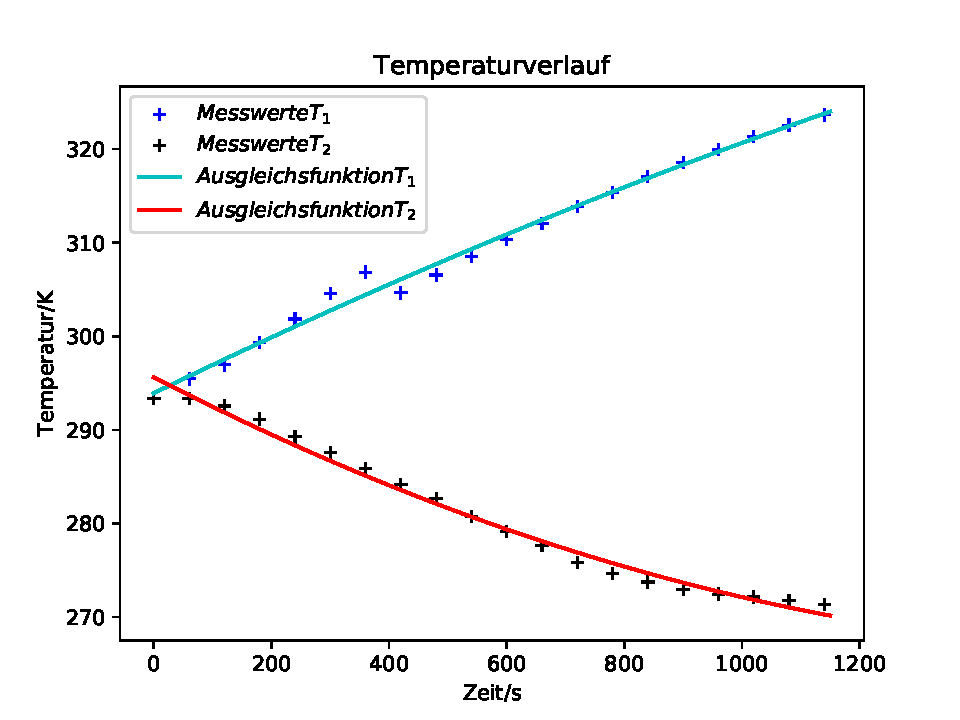
\includegraphics[width=\textwidth]{temp.pdf}
   \caption{Temperaturverläufe}
   \label{fig:temp}
 \end{figure}

\subsection{Differentialquotient unterschiedicher Temperaturen}
\begin{equation*}
  \frac{dT(t)}{dt} = 2At +B\, \,  := f
\end{equation*}

\begin{table}
  \centering
  \caption{Differentialquotieten}
  \label{tab:1}
  \begin{tabular}{c c c c c }
    \toprule $Zeit[s]$ & $T_1[K]$ & $\frac{dT_1}{dt}$ & $T_2[K]$ & $\frac{dT_2}{dt}$ \\
    \midrule
    120 & 296,95 & (0,0297\pm 0,0023)  & 292,55 & (-0,0303\pm 0,0024) \\
    300 & 304,55 & (0,0283\pm 0,0026)  & 287,55 & (-0,0271\pm 0,0027) \\
    600 & 310,35 & (0,0260 \pm 0,0033) & 279,15 & (-0,0217\pm 0,0034) \\
    1080& 322,55 & (0,022 \pm 0,005)   & 271,75 & (-0,013\pm 0,005)\\
    \bottomrule
  \end{tabular}
\end{table}
Die Fehler zu den Quotienten bestimmen sich mit Formel:
\begin{equation}
  \Delta f = \sqrt{(2t\cdot \Delta A)^2 + \Delta B^2}
\end{equation}

\subsection{Güteziffer}

Mit den Formeln (\ref{eqn:Gue}) und (\ref{eqn:nu}) kann die reale Güteziffer berechnet werden.
es ergibt sich die Formel:
\begin{equation*}
  \nu _{real} = (m_wc_w+m_kc_k)\cdot \frac{dT_1}{dt}\cdot \frac{1}{N}
\end{equation*}
Der $m_kc_k$-Wert ist an der apparatur abzulesen und beträgt $660$ J/K.\\
Der $c_w$-Wert beträgt $4,182$ kJ/kgK.\cite[272]{b1}\\
Der $m_w$-Wert ist durch das Reservoire gegeben, das mit drei Litern befüllt wurde.
Smit ergibt sich:
\begin{equation*}
  c_wm_w  = 12546 \frac{J}{K}
\end{equation*}
Die ideale Güteziffer wird mit Formel (\ref{eqn:id}) bestimmt.
\begin{table}
  \centering
  \caption{reale und ideale Güteziffern}
  \label{tab:1}
  \begin{tabular}{c c c c c c}
    \toprule $Zeit[s]$ & $N[W]$ & $T_1[K]$ & $T_2[K]$ & $\nu _{ideal}$ &
    $\nu _{real}$ \\
    \midrule
    120 & 185 & 296,95 & 292,55 & 67,489 & (2,1 \pm 0,16)\\
    300 & 204 & 304,55 & 287,55 & 17,914 & (2,02\pm 0,19)\\
    600 & 210 & 310,35 & 279,15 &  9,947 & (1,86\pm 0,24)\\
    1080& 204 & 322,55 & 271,75 &  6,349 & (1,6 \pm 0,4)\\
    \bottomrule
  \end{tabular}
\end{table}
Die Fehler für $\nu _{real}$ berechnen sich mit der Formel
\begin{equation*}
  \Delta \nu = \left|\left(m_wc_w + m_kc_k\right)\frac{1}{N}\cdot\left(\Delta\frac{dT_1}{dt}\right)\right|
\end{equation*}
\newpage
\subsection{Massendurchsatz des Transportgases}
Um den Massendurchsatz bestimmen zu können muss zunächst die Verdampfungswärme $L$ bestimmt werden.
Dies geschieht durch eine Ausgleichsgerade. Dafür wird $ln(p)$ gegen $1/T$ aufgetragen.
Aus der Formel
\begin{equation*}
  ln(p) = \frac{L}{R}\cdot \frac{1}{T}
\end{equation*}
und der Ausgleichsfunktion
\begin{equation*}
  f(x) = a\cdot x +b
\end{equation*}
folgt der Zusammenhang
\begin{equation*}
  L = -a\cdot R\, .
\end{equation*}
Dabei ist $R$ die allgemeine Gaskonstanteund a der Parameter,
der Aus der Dampfdruckkurve gewonnen wird. Diese ist in abbildung (\ref{fig:Dampf})zu finden.
Die lineare Ausgleichsrechnung wurde mit Python durchgeführt. Mit
\begin{equation*}
  f(x) = a\cdot x+b
\end{equation*}
ergeben sich
\begin{align}
  a &= (-2,23 \pm0,14)\cdot 10^3 \, \mathrm{K} \\
  b &= (9,5 \pm 0,5)
\end{align}
\begin{figure}
  \centering
  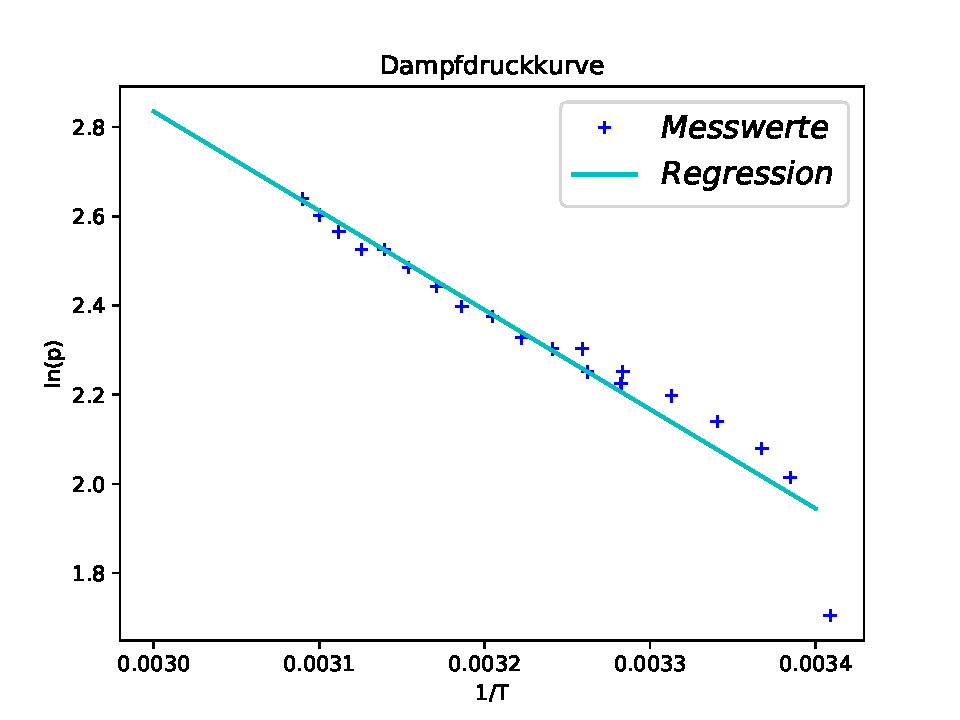
\includegraphics[width=\textwidth]{verd.pdf}
  \caption{Dampfdruckkurve}
  \label{fig:Dampf}
\end{figure}

Mit $R = 8,3144621$ J/molK\cite{b1} folgt für L:
\begin{equation*}
  L = (1,85\pm 0,12)\cdot 10^4\, \mathrm{\frac{J}{mol}}
\end{equation*}
Der Fehler berechnet sich durch:
\begin{equation*}
  \Delta L = R\cdot \Delta a
\end{equation*}
Mit den Formeln (\ref{eqn:masds}) und (\ref{eqn:msds}) kann nun der Massendurchsatz ermittelt werden:
\begin{equation*}
  \frac{dm}{dt} = \frac{1}{L}(m_wc_w + m_kc_k)\frac{dT_2}{dt}
\end{equation*}
Der Fehler berechnet sich durch:
\begin{equation*}
  \Delta \left(\frac{dm}{dt}\right) = \sqrt{\left(\frac{1}{L}(m_wc_w + m_kc_k)\cdot\left(\Delta\frac{dT_2}{dt}\right)\right)^2
  + \left(\frac{-1}{L^2}(m_wc_w + m_kc_k)\frac{dT_2}{dt}\cdot \Delta L\right)^2}
\end{equation*}
Die ergebnisse sind in Tabelle (\ref{tab:msd}) zu finden.
Da der Massendurchsatz in mol/s angegeben ist, wird er in g/s umgerechnet.
Dies geschieht, indem die molare Masse hinzu multipliziert wird.
Sie beträgt $102,92$ g/mol.\cite{on2}
\begin{table}
  \centering
  \caption{Massendurchsatz}
  \label{tab:msd}
  \begin{tabular}{c c c}
    \toprule $Zeit[s]$ & $dm/dt[mol/s]$ & $dm/dt[g/s]$ \\
    \midrule
    120 & (-0,0216 \pm 0,0022)  & (-2,223 \pm 0,226)\\
    300 & (-0,0193 \pm 0,0023)  & (-1,986 \pm 0,237)\\
    600 & (-0,0155 \pm 0,0026)  & (-1,595 \pm 0,268)\\
    1080& (-0,009 \pm 0,004)    & (-0,926 \pm 0,412)\\
    \bottomrule
  \end{tabular}
\end{table}

\subsection{mechanische Leistung des Kompressors}
Die mechanische Leistung wird mit Formel (\ref{eqn:Nmech}) bestimmt.
Aus der idealen Gasgleichung
\begin{equation*}
  p\cdot V = R\cdot m\cdot T
\end{equation*}
und
\begin{equation*}
  V =\frac{m}{\rho}
\end{equation*}
folgt für die Dichte:
\begin{equation*}
  \rho = \frac{\rho _0T_0p_a}{p_0T_2}\, .
\end{equation*}
Vorher gegeben sind:
\begin{align*}
  \rho _0 &= 5,51\cdot 10^{-3} \,\mathrm{\frac{kg}{L}}\\
  T &= 273,15 \, \mathrm{K} \\
  p &= 1\, \mathrm{Bar} = 10^4 \, \mathrm{Pa}\\
  \kappa &= 1,14
\end{align*}
\cite{on1}\\

Der Fehler berechnet sich mit der Formel
\begin{equation*}
  \Delta  N = \frac{1}{\kappa - 1} \left( p_b \sqrt[\kappa]{\frac{p_a}{p_b}} - p_a \right)
  \frac{1}{\rho}\cdot \Delta \left(\frac{dm}{dt}\right)\, .
\end{equation*}
Die Ergebnisse sind in Tabelle (\ref{tab:mech}) zu finden.
\begin{table}
  \centering
  \caption{Mechanische Leistung}
  \label{tab:mech}
  \begin{tabular}{c c c c}
    \toprule $Zeit[s]$ & $\rho [kg/m^{3}]$ & $\sqrt{p_a/p_b}$ & $N_{mech}[W]$  \\
    \midrule
    120 & 15,43 & 0,42300 & (-4,0 \pm 0,4) \\
    300 & 16,23 & 0,37443 & (-4,0 \pm 0,5) \\
    600 & 16,71 & 0,35028 & (-3,3 \pm 0,6) \\
    1080& 17,17 & 0,27510 & (-2,4 \pm 1,1)  \\
    \bottomrule
  \end{tabular}
\end{table}

\section{Disskusion}
Werden die beiden Temperaturverläufe in Abbildung (\ref{fig:temp}) betrachtet,
ist ein Sprung in den Messwerten vom Reservoire 1 zu sehen.
Dieser entstand durch einen Defekt des Versuchsaufbaus.
Die Heizspule im Inneren des Behälters drehte sich nicht mehr selbstständig,
sodass das Wasser nicht gleichmäßig erhitzt wurde.
Nach sechs Minuten wurde per Hand gedreht,
sodass sich das Wasser vermischen konnte und der Sprung in den Messwerten entstand.
Dieser Sprung ist auch in der Verdampfungskurve in Abbildung (\ref{fig:Dampf}) gut zu sehen.
Es ist zu sehen, dass die reale Güteziffer viel kleiner ist als der ideale Wert.
Es wird davon ausgegangen, dass der Kompressor adibatisch ist. Das ist so nicht möglich.
Beim idealen Wert wird außerdem von einer verlustfreien Isolierung ausgegangen,
dies ist an dem Versuchsaufbau aber nicht komplett umsetztbar, sodass es hier zu Verlusten kommt.
Der Wärmeaustausch der Reservoire mit der Umgebung kann nicht komplett verhindert werden.
Somit kommt es zu Druckverlusten bzw. -zunahmen.
Dies hat also auch Einfluss auf die Verdampfungswärme und somit auf den Massendurchsatz.
Der negative Wert für den Massendurchsatz ist zu erklären,
indem man den Temperaturverlauf von $T_2$ betrachtet.
Der Wert ist von dem negativen Parameter abhängig.
